\begin{figure}[H]

	\centering
	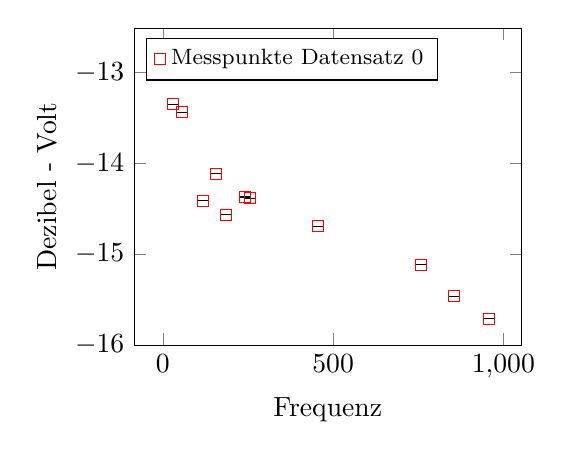
\begin{tikzpicture}
		\pgfplotsset{width=6.5cm,compat=1.3,legend style={font=\footnotesize}}
		\begin{axis}[xlabel={Frequenz},ylabel={Dezibel - Volt},legend cell align=left,legend pos=north west]
		
\addplot+[only marks,color=red,mark=square,error bars/.cd,x dir=both,x explicit,y dir=both,y explicit,error bar style={color=black}] table[x=X,y=Y,x error=xerror,y error=yerror,row sep=\\]{
			X	Y	xerror	yerror	\\
			 10.253906 	 -12.80232 	 0 	 0 	\\
			 30.761719 	 -13.347933 	 0 	 0 	\\
			 57.128906 	 -13.436821 	 0 	 0 	\\
			 118.652344 	 -14.413613 	 0 	 0 	\\
			 156.738281 	 -14.114061 	 0 	 0 	\\
			 184.570312 	 -14.565412 	 0 	 0 	\\
			 241.699219 	 -14.37053 	 0 	 0 	\\
			 254.882812 	 -14.385941 	 0 	 0 	\\
			 455.566406 	 -14.692671 	 0 	 0 	\\
			 757.324219 	 -15.117664 	 0 	 0 	\\
			 855.46875 	 -15.462831 	 0 	 0 	\\
			 958.007812 	 -15.711401 	 0 	 0 	\\
		};
		\addlegendentry{Messpunkte Datensatz 0}

		\end{axis}
		\end{tikzpicture}
	\caption{Umgebung}
	\label{fig:Umgebungsmessung}
\end{figure}
